\hyphenation{diffe-rent}
%%%%%%%%%%%%%%%%%%%%% Conclusions %%%%%%%%%%%%%%%%%
\chapter{Conclusions}
\label{ch:Conclusions}

\section[Search for production of a Higgs boson and a single top quark]{Search for production of a Higgs boson and a single top quark in multilepton final states in pp collisions at $\sqrt{s}$ = 13 TeV}

In this thesis, a search for the production of a Higgs boson in association with a single top quark has been presented, using the CMS detector and the full 2016 data sample of \pp collisions at $\sqrt{s}=13$ TeV, corresponding to an integrated luminosity of 35.9 ~\fbinv. Three channels have been analyzed, looking at the Higgs boson decaying to a pair of W or Z bosons, or two $\tau$ leptons and the leptonic decay of the top: two same-sign leptons ($\mu\mu, e\mu$) and three leptons. This process benefits from an enhancement in the production cross section in the case of anomalous top-Higgs couplings and the results are used to constrain these couplings.

The analysis was performed on the basis of the existing analysis \ti{Search for \ttH in multilepton final states at $\sqrt{s}=13$} TeV \cite{CMS_AN_2017-029}, to which several elements were added: a dedicated signal discrimination strategy based on multivariate analysis, implemented through the usage of boosted decision trees (BDT) which, after a parameter optimization process, showed a better performance compared to several other discriminators like Fisher and K-NN methods. A binned shape fitting on the BDT output was used to extract the signal. The main addition was the interpretation of the results in terms of the ratio of the coupling modifiers (\Ct,\CV), which differs from previous \tH analyses and even from the base \ttH analysis; therefore, it was necessary to adapt the systematic uncertainties and background estimations.

Combining the results from all three channels yields a 95\% confidence level (C.L.) upper limit on the production cross section times branching ratio of events containing a SM Higgs boson of 0.56 pb; the expected limit is 0.24 pb. In the case of the inverted top-Higgs coupling a combined upper limit on the production cross section times branching ratio of 0.64 pb has been set with an expected limit of 0.32 pb.  

Values of the ratio of top-Higgs coupling modifier \Ct and Higgs-vector boson coupling modifier \CV that are outside the range -1.25 to +1.60 are excluded at 95\% C.L for \CV=1.0, which is in agreement with the SM predictions. These results of the analysis have been made public by the CMS collaboration in an analysis note \cite{CMS_AN_2016-378} and a Physics Analysis Summary \cite{CMS_PAS_HIG_17-005}.

The sensitivity of the \tH process to the CP-mixing phase angle ($\alpha_{CP}$) in the Higgs sector was investigated under the assumption of a generic spin-0 particle $X_0$ with CP-symmetry violating interaction with the top quark but SM-like interaction with the W boson, by using Monte Carlo samples generated for several Higgs boson coupling configurations, including the SM scenario ($\cos(\alpha_{CP})$=1) and the ITC scenario ($\cos (\alpha_{CP})$=-1).  

Combining the results from all three channels yields a 95\% confidence level (C.L.) upper limit on the production cross section times branching ratio of events containing a SM Higgs boson of 0.55 pb has been set, while for the case of the ITC scenario a combined upper limit on the production cross section times branching ratio of 0.60 pb has been set; the expected limits are 0.30 pb and 0.24. These limits are in agreement with the results from the \Ct/\CV study; however, in the CP-mixing case it is not possible to exclude any region/value in the $\alpha_{CP}$ phase space.

Currently, a combination with the \tH analysis in the $H \to b\bar{b}$ Higgs decay channel and with a reinterpretation of the \ttH result in the $H\to \gamma\gamma$ decay channel is in preparation for publication.

The sensitivity of the analysis is limited by systematic uncertainties, mainly by those associated to the normalizations of the major background components, \ie, the non-prompt lepton estimation, the scale uncertainties for \ttW and \ttZ, as well as by the uncertainties on the measured lepton efficiency. In the future refinements of the analysis,  the reduction of the systematic uncertainties will be a crucial aspect. In addition, increasing the amount of data analized will allows for a better background contraining, by increasing the number of bins in the final S/B ratio map, so that the dominance of backgrounds can be well stablished by regions and then be better constrained.       
 
\section{Phase 1 FPix upgrade module production}

Building a detector involves many challenges, and the HEP group at UNL accepted the leading role of assembling the modules that compose the forward pixel detector of the CMS detector at CERN. The commissioning of the full pixel module production line started from scratch in late 2012 and by 2015 the same yield level as highly experienced groups was reached; this by itself is a big achievement given the leading role assumed by the students involved. %As a result, the two modules installed in the pilot in 2015 were assembled at UNL.  

The inclusion of the robotic pick-and-place machine in the assembly provided a shorter production time and uniformity of production assembly technique. In total, 45\% (555) of the FPix modules were assembled at UNL.  

Each stage in the production line went through an optimization process to reduce the assembly time while increasing the quality of the produced modules. In particular, in the gluing and encapsulation stages everything was optimized to be done with one hand, turning out to be more efficient since it involved fewer steps and fewer hands-on touches, increasing the yield of the production.

\clearpage

\section*{CMS-CERN official guide}
\small
Many histories have been told about CERN and the plans of crazy scientist there to destroy the planet, or those relating us with investigations in massive destruction weapons and sacrifices to the dark side; the truth be said, we do more exciting things!, and we are willing to show that to everybody; CERN is visited by about 100.000 people a year and we take them to learn about several installations.

\begin{figure}[h]
     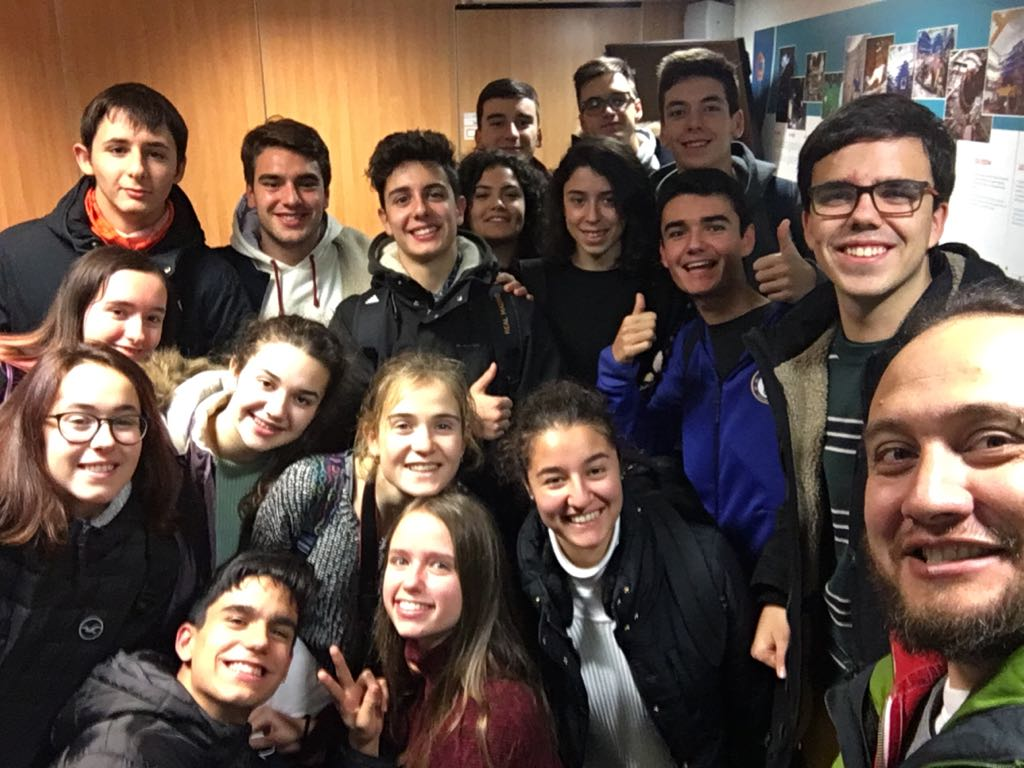
\includegraphics[width=0.24\textwidth,height=0.16\textwidth]{guide/1.png}  
     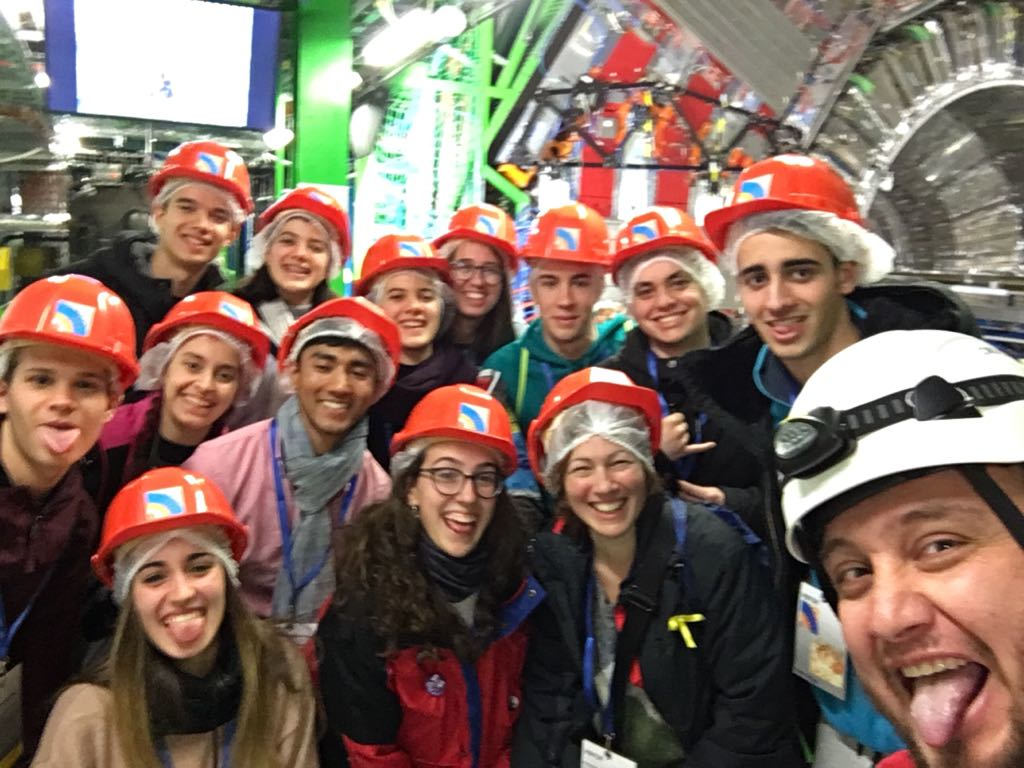
\includegraphics[width=0.24\textwidth,height=0.16\textwidth]{guide/2.png}
     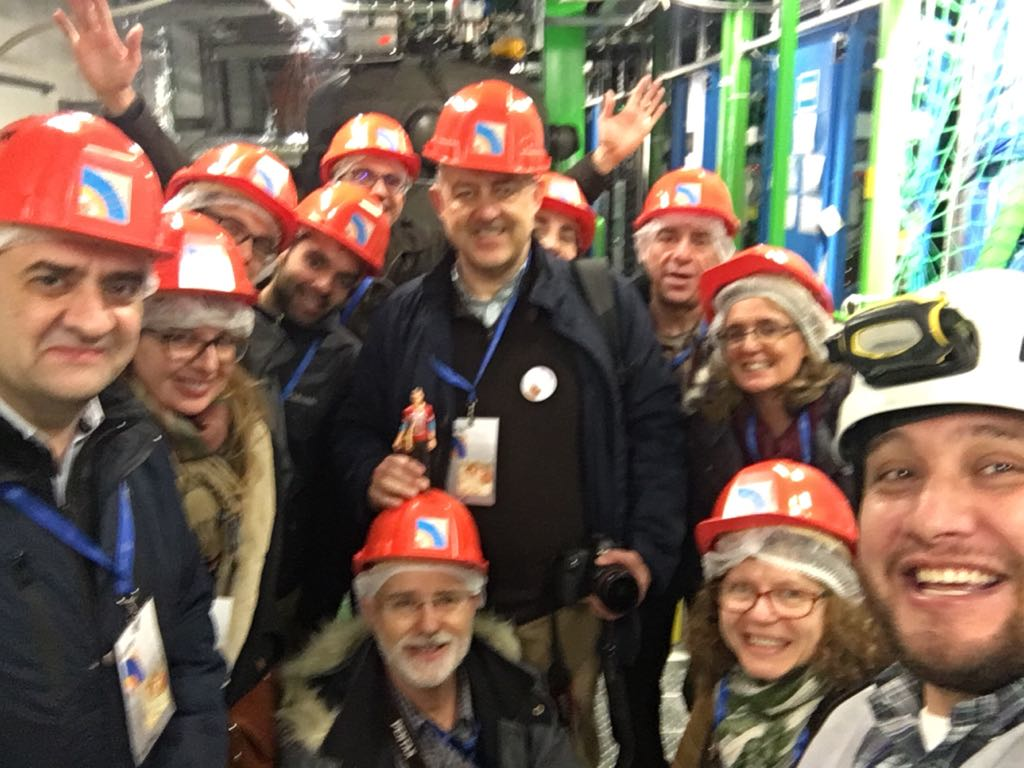
\includegraphics[width=0.24\textwidth,height=0.16\textwidth]{guide/3.png}
     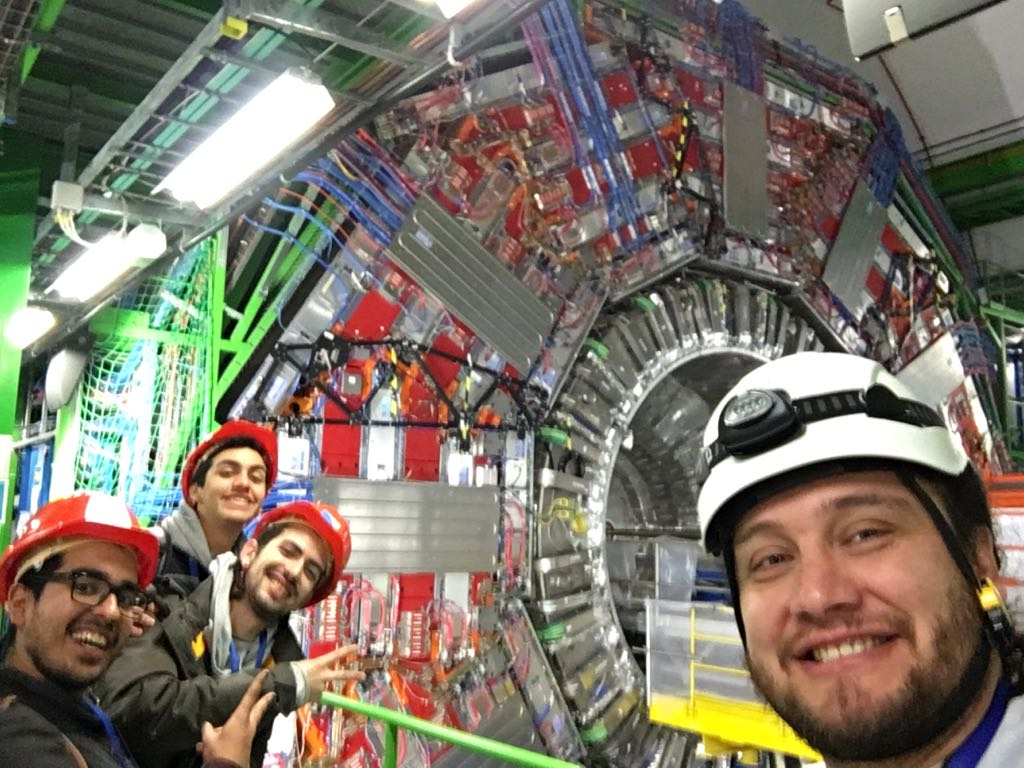
\includegraphics[width=0.24\textwidth,height=0.16\textwidth]{guide/4.png}\\
     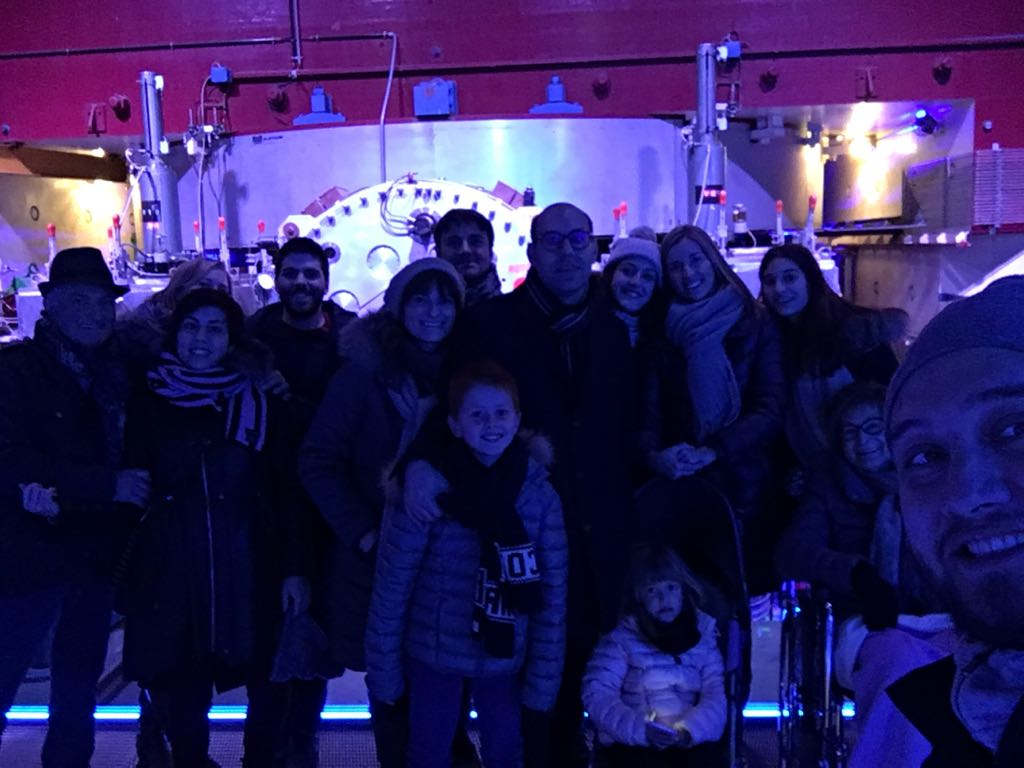
\includegraphics[width=0.24\textwidth,height=0.16\textwidth]{guide/5.png}
     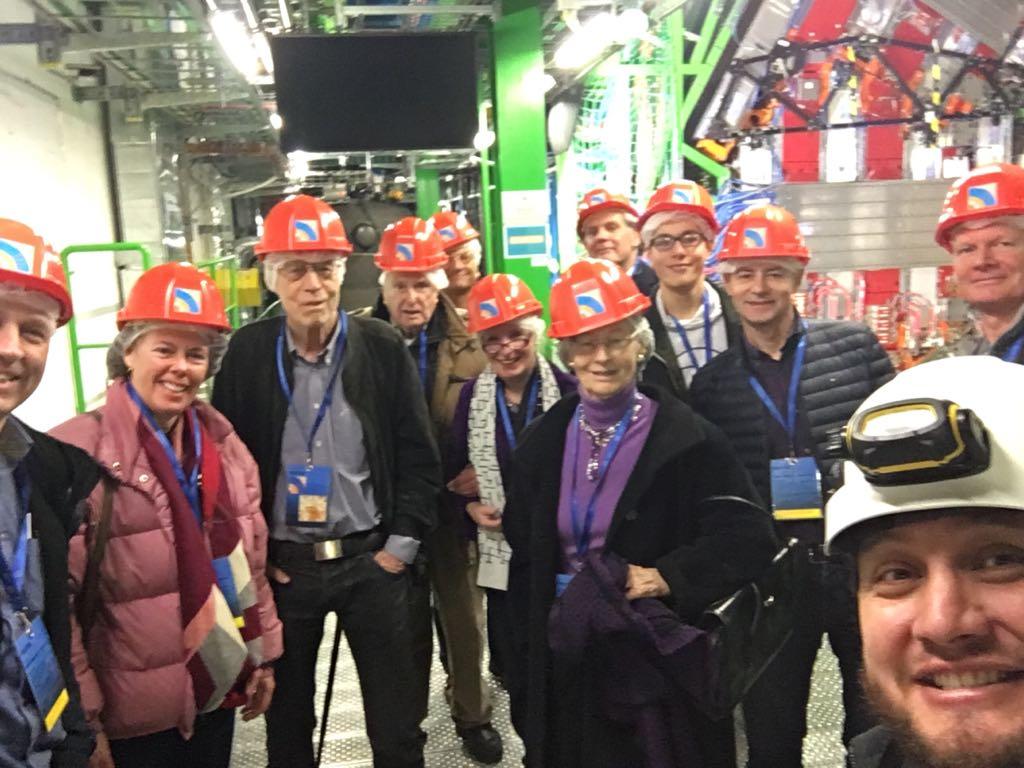
\includegraphics[width=0.24\textwidth,height=0.16\textwidth]{guide/6.png}
     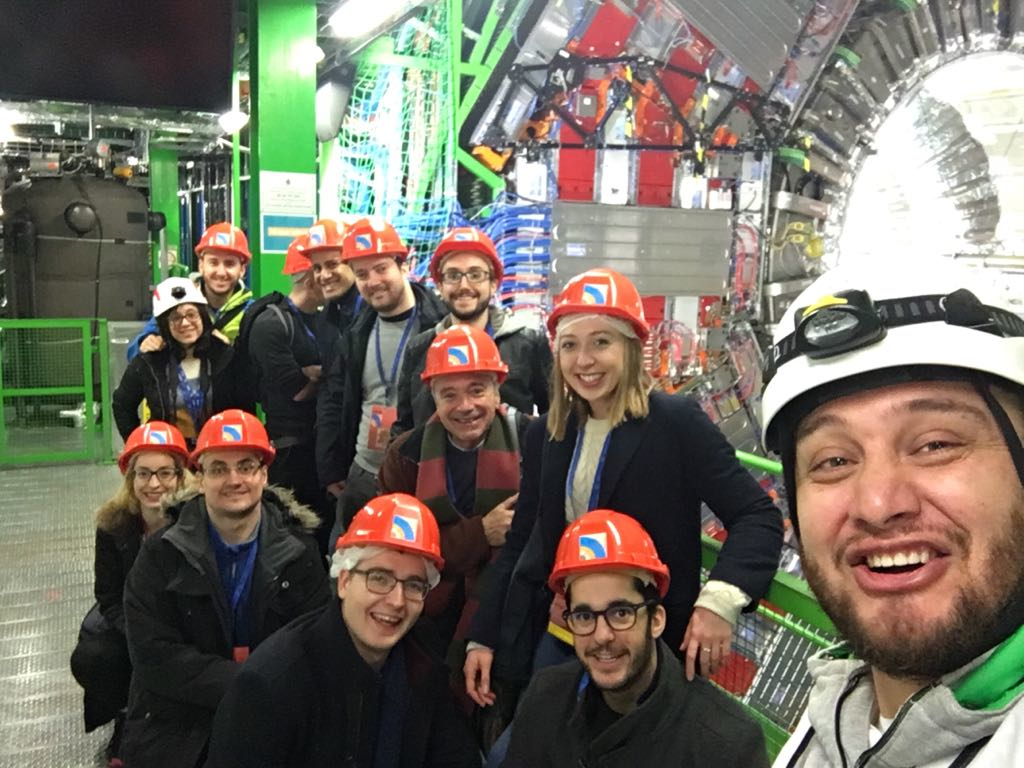
\includegraphics[width=0.24\textwidth,height=0.16\textwidth]{guide/7.png}
     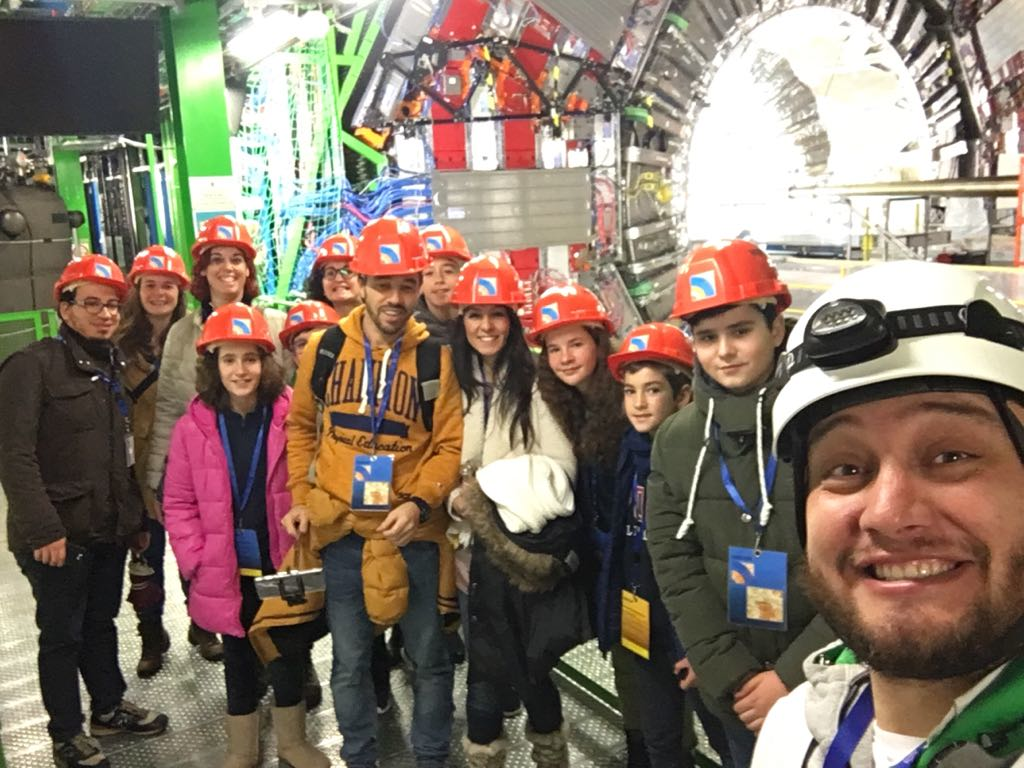
\includegraphics[width=0.24\textwidth,height=0.16\textwidth]{guide/8.png}\\
     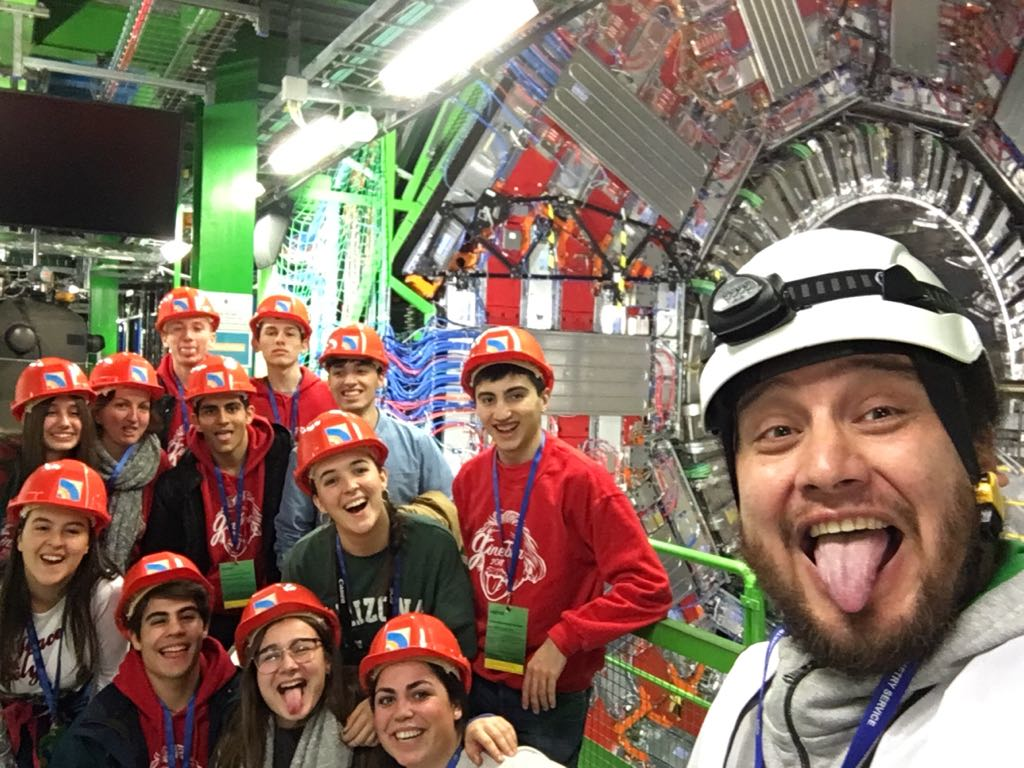
\includegraphics[width=0.24\textwidth,height=0.16\textwidth]{guide/9.png}
     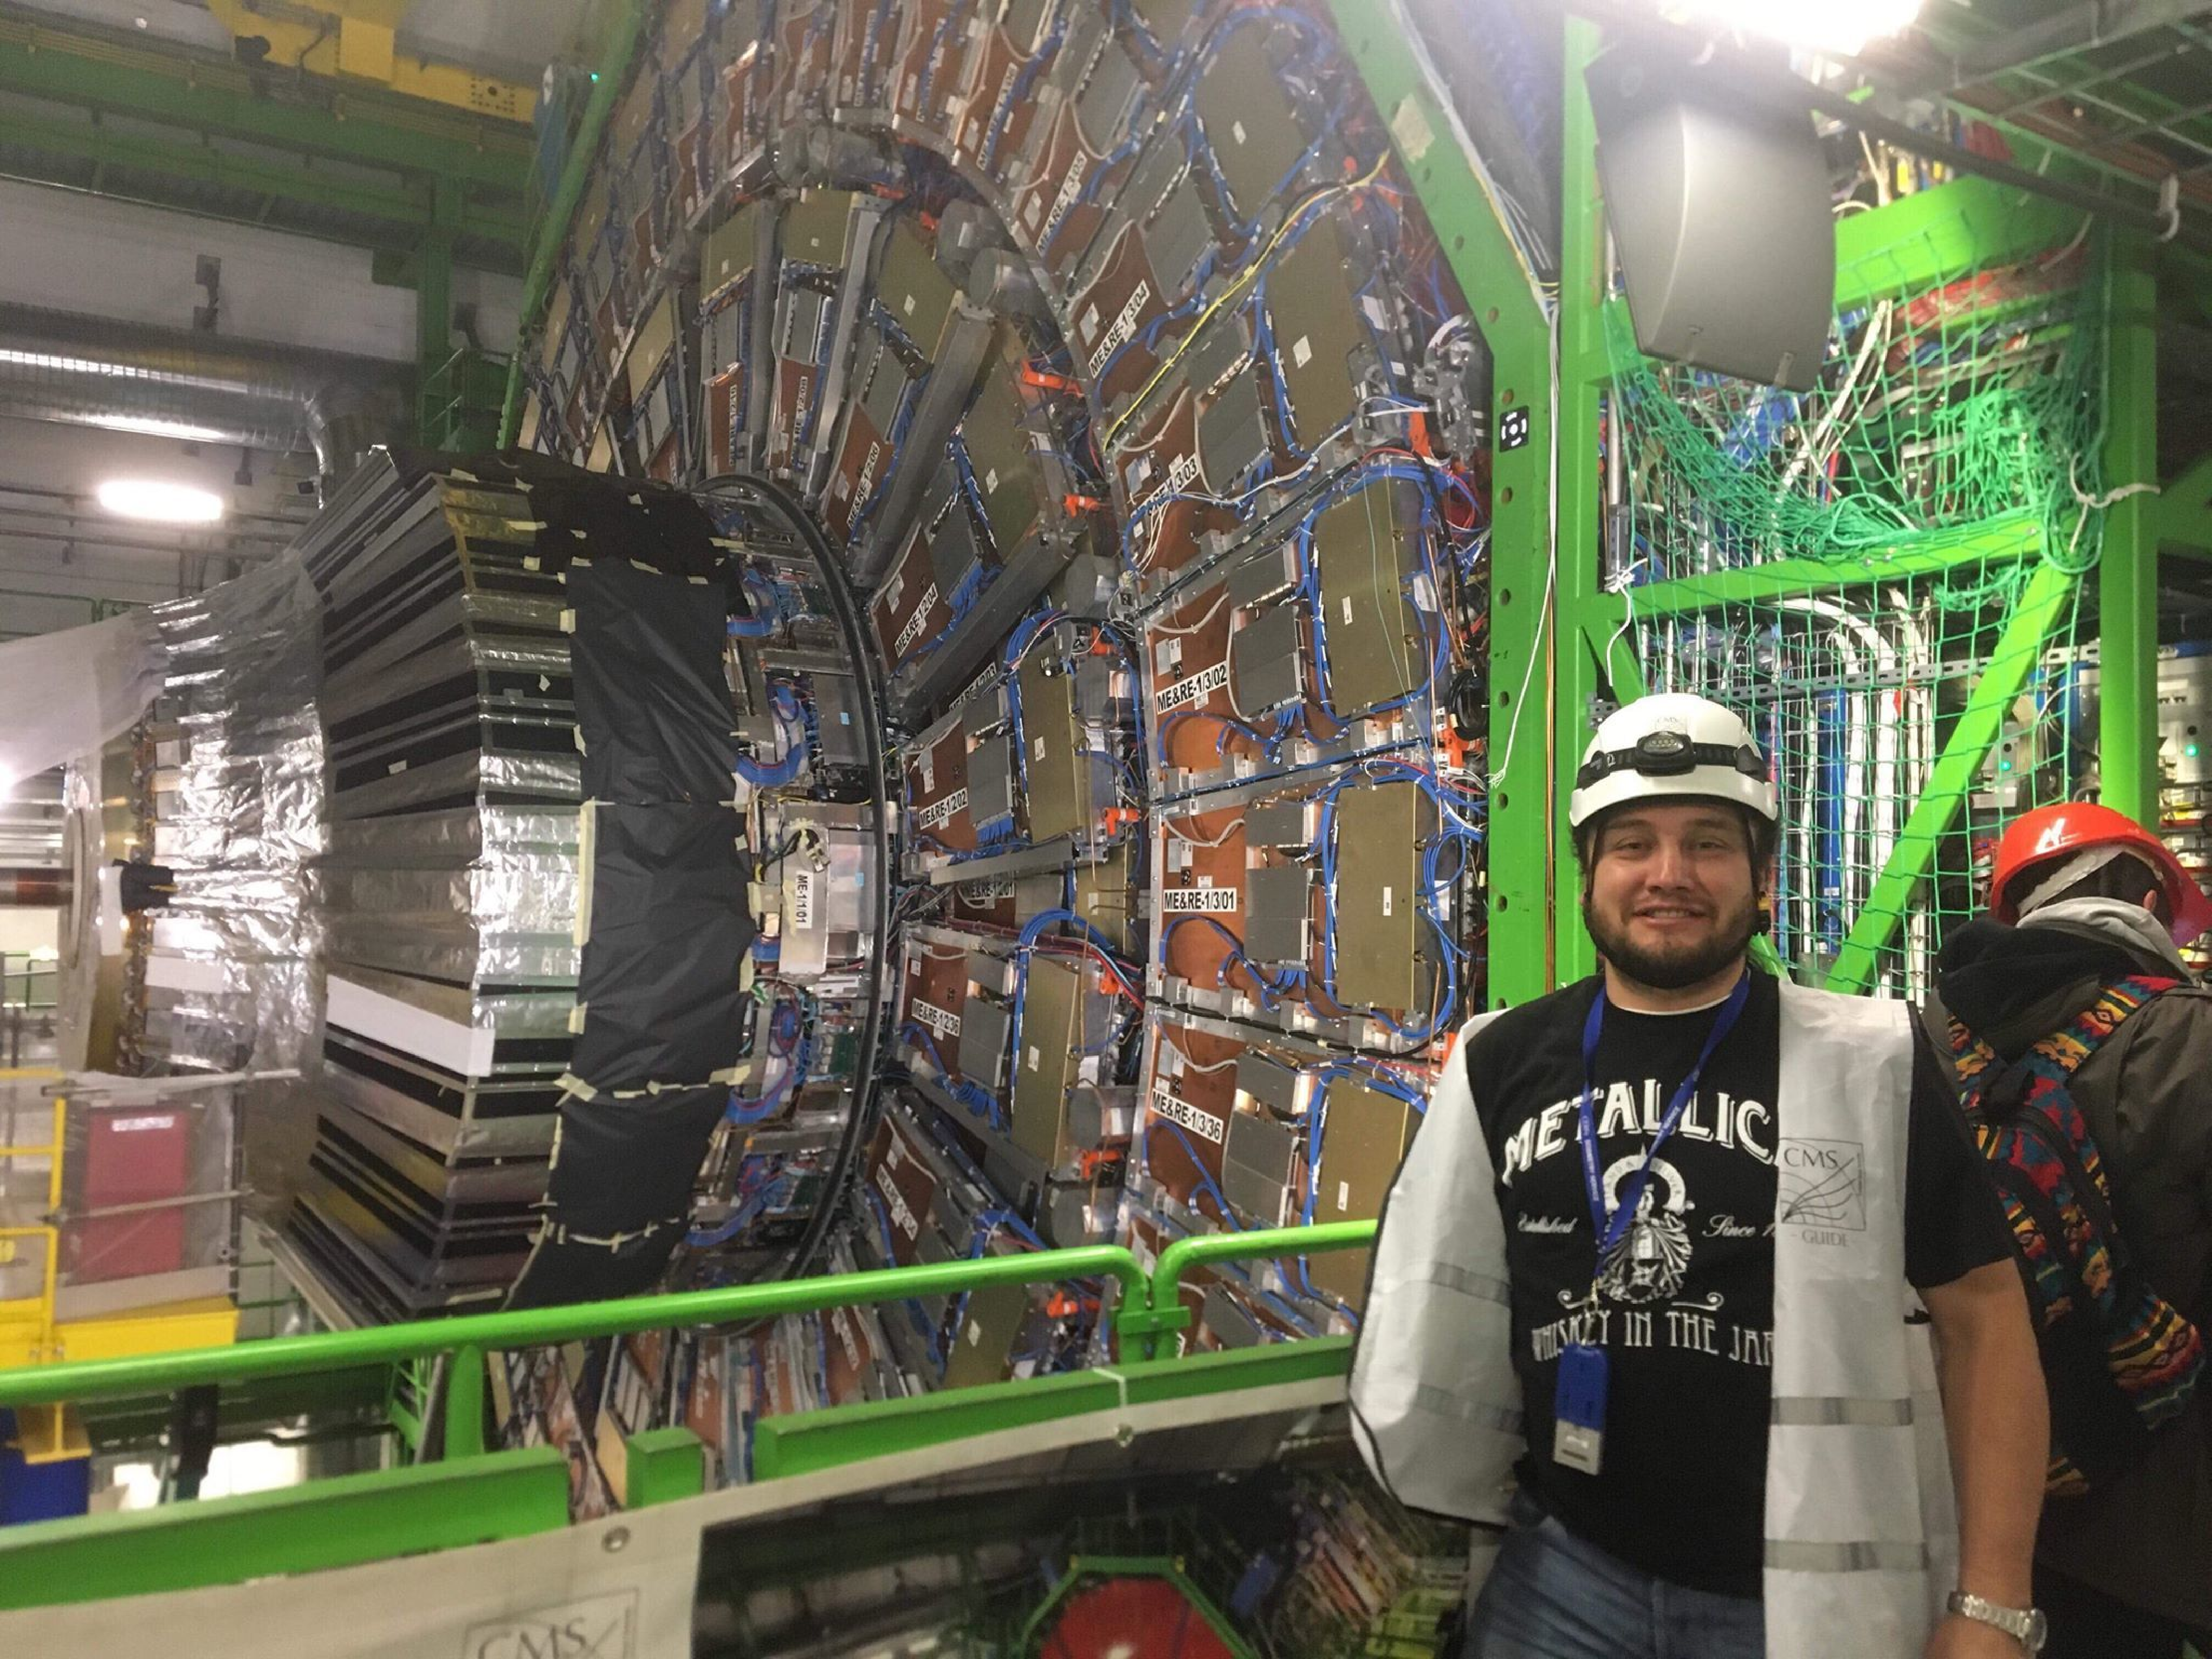
\includegraphics[width=0.24\textwidth,height=0.16\textwidth]{guide/tour.pdf}
     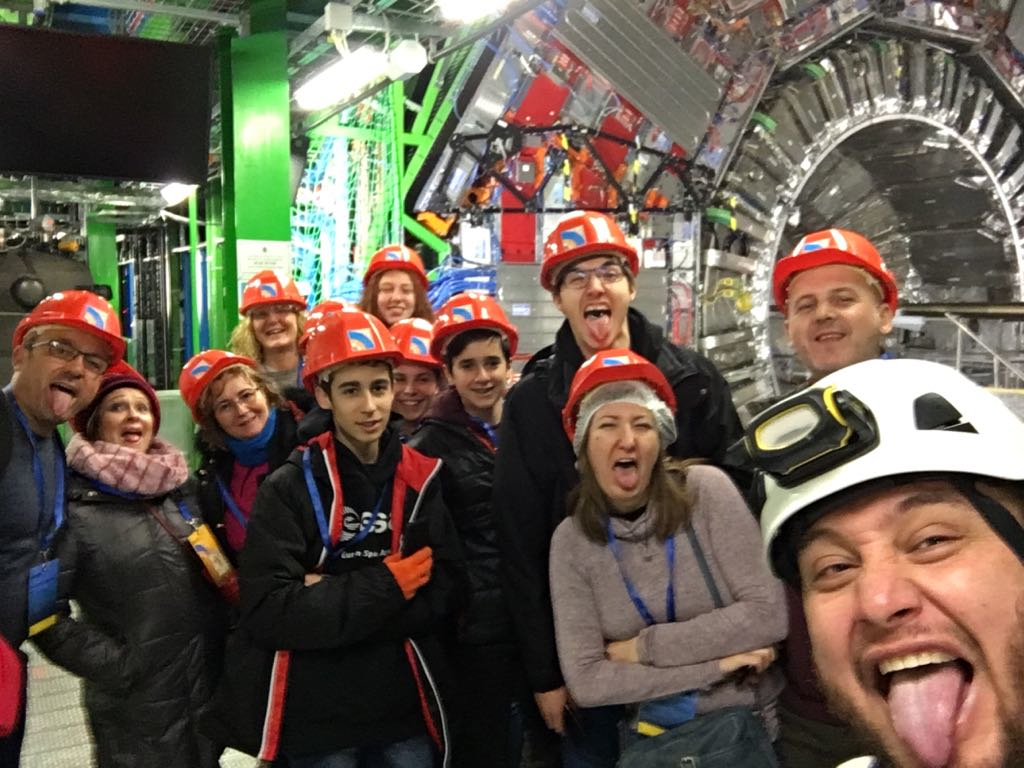
\includegraphics[width=0.24\textwidth,height=0.16\textwidth]{guide/10.png}
     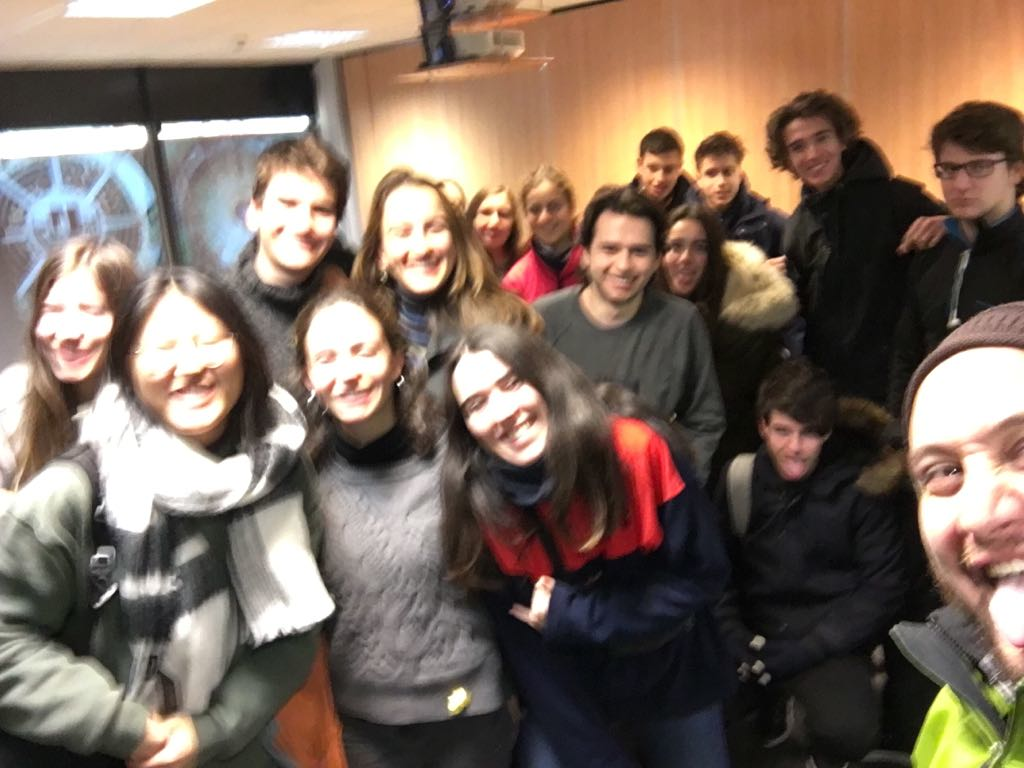
\includegraphics[width=0.24\textwidth,height=0.16\textwidth]{guide/11.png}\\
     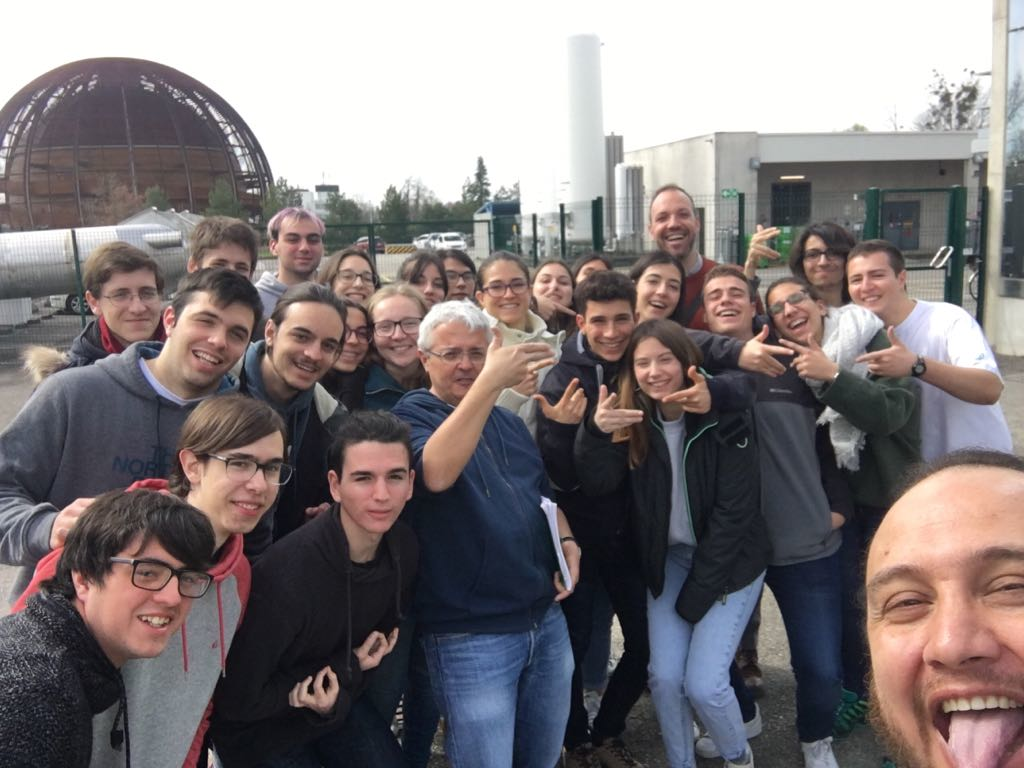
\includegraphics[width=0.24\textwidth,height=0.16\textwidth]{guide/12.png}
     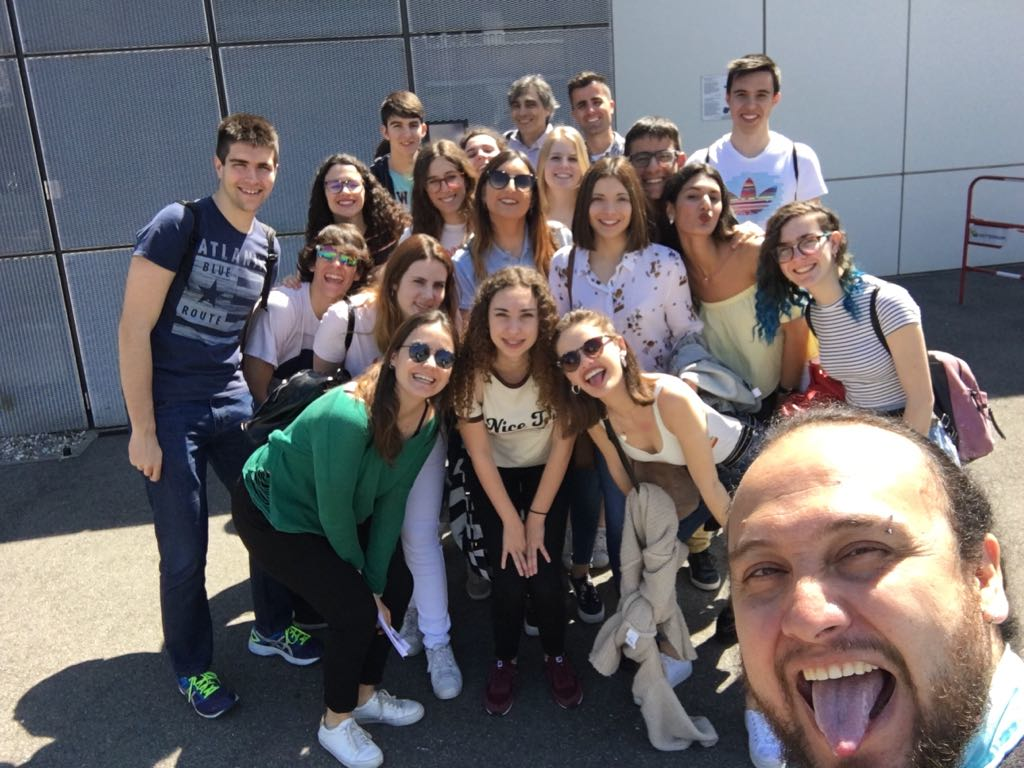
\includegraphics[width=0.24\textwidth,height=0.16\textwidth]{guide/13.png}
     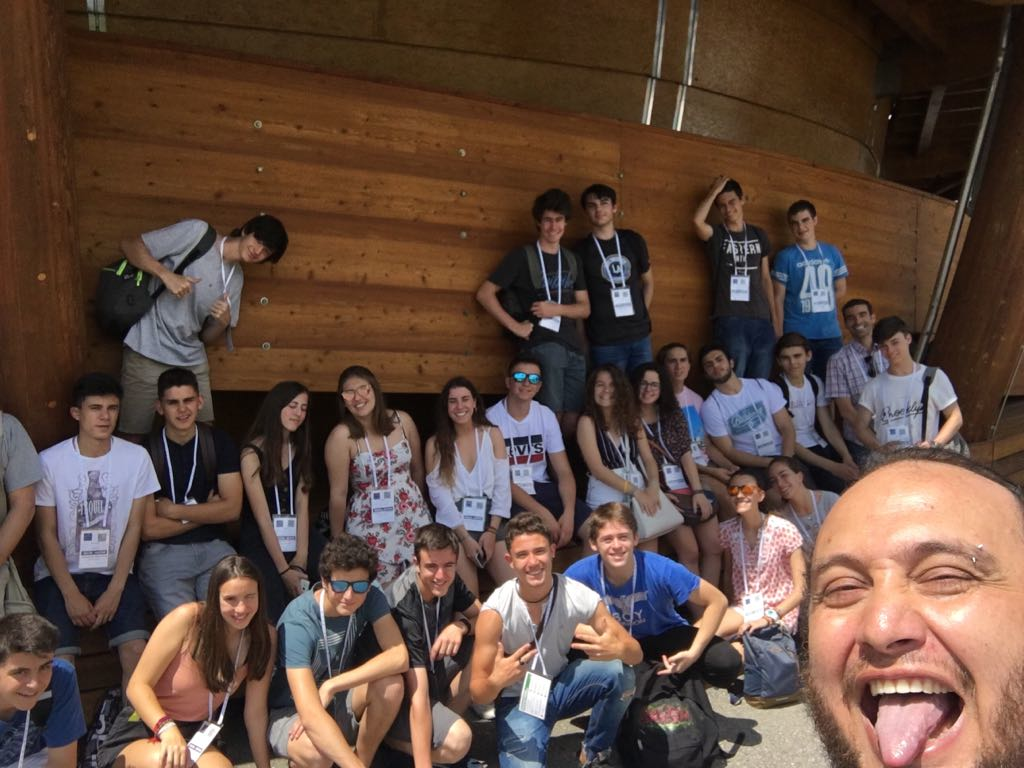
\includegraphics[width=0.24\textwidth,height=0.16\textwidth]{guide/14.png}
     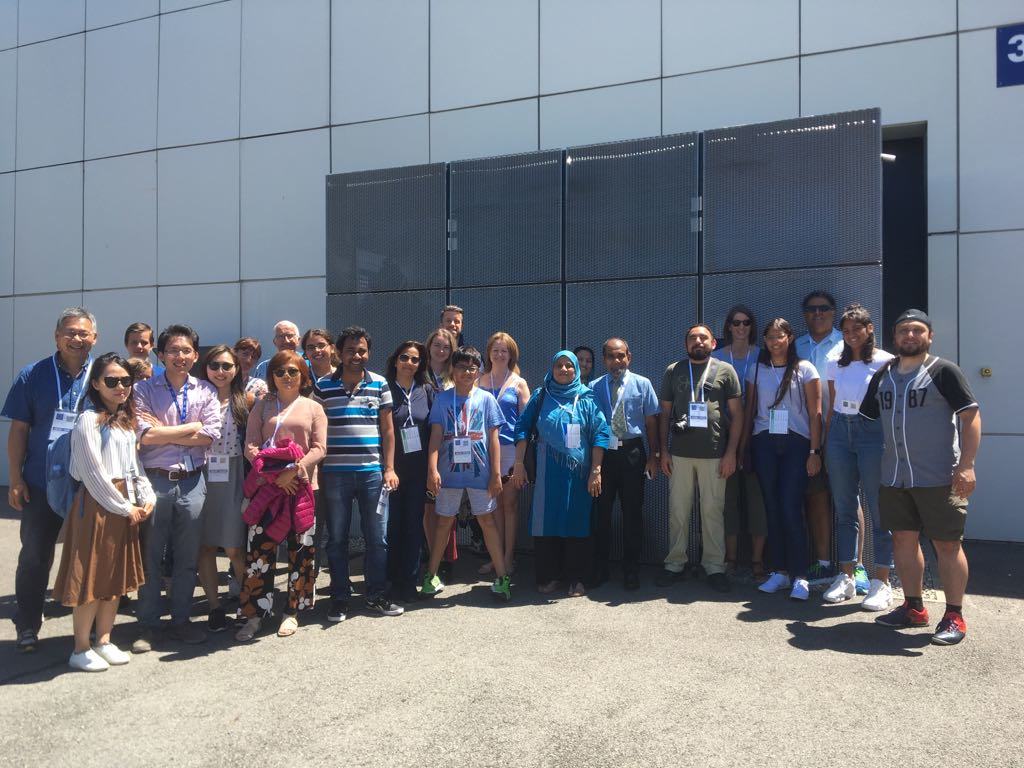
\includegraphics[width=0.24\textwidth,height=0.16\textwidth]{guide/15.png}
   \end{figure}

When I had hard times, fighting against analysis code, and I had forgotten the excitement of the HEP world, it was enough to take a group of enthusiastic people willing to learn about particle physics and show them the most incredible machine ever built - I might be a bit biased here - to recharge courage and feel alive again. The pictures show that they enjoyed the visits and certainly I did it too. It is true, we create black holes and all kind of strange particles! but even in the worst case scenario, if a black hole eat us, we will get a free ride to Switzerland and who does not want to go to Switzerland!     


